\title{Programming Assignment 4}
\author{
	Aditya Gupta\\
	\underline{2015CSB1003}}
\date{\today}
\documentclass{article}
\usepackage{adjustbox}
\usepackage{amsmath}
\usepackage{float}
\usepackage{graphicx}
\begin{document}
\maketitle
\section{Planners for Block World}
\subsection{Introduction}
The goal of this lab was to implement a planning agent for solving Block World Problem wherein given $N$ blocks and actions to ``pick a block from table'', ``unstack a block from another block'', ``release a holding block'' and ``stack a holding block onto another block'' we were required to reach a goal state configuration from an initial state using three different planners, ``forward search planner'' with BFS and A*; ``goal stack planning''. The initial and final state is composed of propositions such as \verb|(on 1 2)| and \verb|(ontable 3)|. Each action is a transformation of these propositions which has some \verb|preconditions|, which when true allows us to perform that action and the \verb|effects| of that actions are unified with the current state and the negative literals removed. States are represented in PDDL.

\section{Forward Search using BFS}
In this search the states are maintained in a queue (initially containing only the initial state) and then every time a element is taken from the queue and checked for satisfying the goals. If it does not satisfy the goals then all actions which are applicable on the current state are taken (after instantiation) and applied on the current state all resulting states pushed onto the queue, in this way we only see states which require equal number of actions from the starting state and we get the optimal solution (minimum number of steps).

\pagebreak
\subsection{Observations}
\begin{itemize}
\item \verb|1.txt| In this problem the planner finds the solution of length 10 in around 3 ms and the optimal solution.

\begin{figure}[H]
    \centering
    \begin{minipage}{0.45\textwidth}
        \centering
        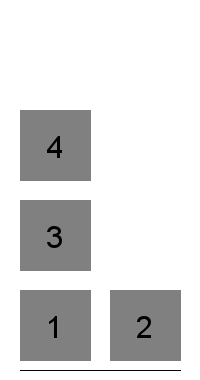
\includegraphics[scale=0.3]{1i}
        \caption{Initial State of 1.txt}
    \end{minipage}\hfill
    \begin{minipage}{0.45\textwidth}
        \centering
        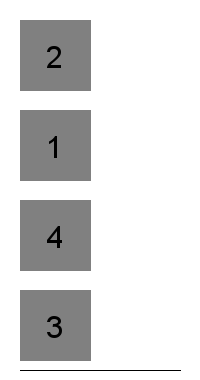
\includegraphics[scale=0.3]{1f}
        \caption{Final State of 1.txt}
    \end{minipage}
\end{figure}

\item \verb|4.txt| In this problem the planner finds the solution of length 14 in around 10ms and the optimal solution.

\begin{figure}[H]
    \centering
    \begin{minipage}{0.45\textwidth}
        \centering
        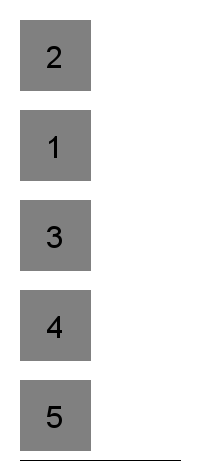
\includegraphics[scale=0.3]{4i}
        \caption{Initial State of 4.txt}
    \end{minipage}\hfill
    \begin{minipage}{0.45\textwidth}
        \centering
        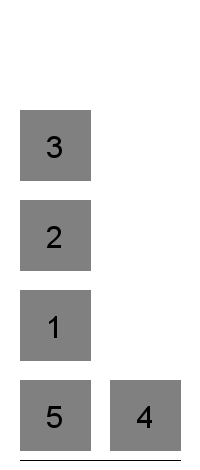
\includegraphics[scale=0.3]{4f}
        \caption{Final State  of 4.txt}
    \end{minipage}
\end{figure}
\end{itemize}

\section{Forward Search using A*}
In this search the planner uses a priority queue instead of a normal queue where the the node with least $f$ value is taken where $f$ is given by:
$$f(n)=g(n)+h(n)$$
where $g$ is the level or depth of the current state, i.e. the total number of nodes takn until now and $h$ is the heuristic function. The heuristic function enables the search to be more directed towards the goal state and is faster and better than BFS. An optimal solution is returned only if the heuristic is admissible.
\subsection{Heuristic Function}
\subsubsection{An Optimal One: Heights of Blocks}
In this heuristic the heights of the blocks in the current state is calculated. This is done via the following way:
\begin{itemize}
\item All the blocks on the table are given height 0, this can be done via finding propositions of type \verb|ontable b|.
\item For all possible blocks the block on it's top is found out and stored, this can be done via finding propositions of type \verb|on a b|
\item Finally the heights of all the blocks are given by starting with the ones on the ground via a BFS.
\end{itemize}
Now we relax the problem in this way: We can move any block from any height to its goal height by first holding it and then putting it, in most cases we either need to clear blocks from top of this or clear blocks on top of the goal block assuming it is in its correct position. So instead of taking these numerous steps we account for only 2 steps which will infact be the minimum. Also if we are holding a block currently we are halfway done so we only add 1 step. The heuristic value is thus the sum of 2 times blocks not currently at their goal height and 1 if we are holding a block.
\subsubsection{An Unoptimal One: Relating to Number of Propositions}
\pagebreak
\subsection{Observations}
\begin{itemize}
\item \verb|1.txt| In this problem the first heuristic finds the solution of length 10 in again around 3ms and the optimal solution whereas the second heuristic finds the solution of length x in y ms which is not the optimal solution.(\textbf{Initial and final state same as} \verb|1.txt|)

\item \verb|6.txt| In this problem the first heuristic finds the solution of length 26 in around 4 min 4s and the optimal solution whereas the second heuristic finds the solution of length x in y ms which is not the optimal solution.

\begin{figure}[H]
    \centering
    \begin{minipage}{0.5\textwidth}
        \centering
        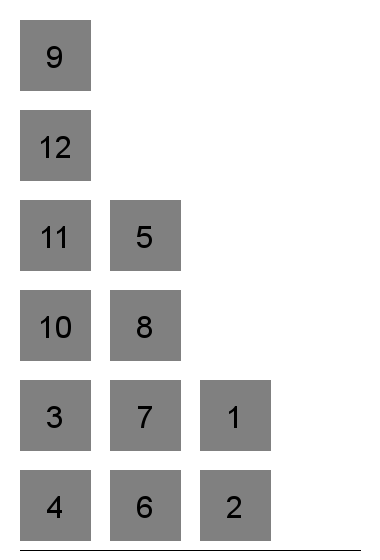
\includegraphics[scale=0.3]{6i}
        \caption{Initial State  of 6.txt}
    \end{minipage}\hfill
    \begin{minipage}{0.5\textwidth}
        \centering
        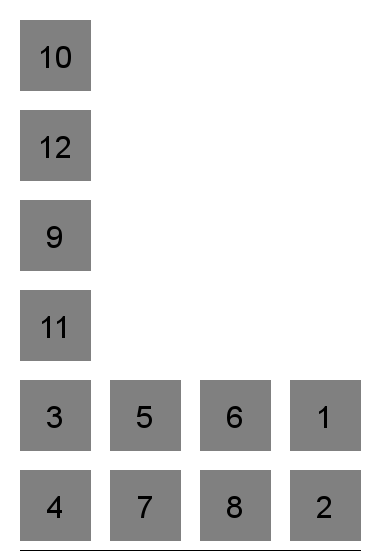
\includegraphics[scale=0.3]{6f}
        \caption{Final State  of 6.txt}
    \end{minipage}
\end{figure}
\end{itemize}

\section{Goal Stack Planning}


\end{document}
